\begin{savequote}[75mm]
Basic research is what I am doing when I don't know what I am doing.
\qauthor{Wernher von Braun}
\end{savequote}

\chapter{$H\rightarrow WW^{*}\rightarrow \ell\nu\ell\nu$ Analysis Strategy}
\label{chap:hwwstrategy}

\section{Introduction}

This chapter presents an overview of the strategy for searching for a Higgs boson in the 
\HWWfull decay topology. Its purpose is to define in broad terms how the search and measurement are undertaken, before going into details on the specific sub-categories within the larger analysis. First, the properties of the Higgs signal are discussed and the associated backgrounds are
presented. Next, the observables used to enhance the signal to background ratio are defined. 
Finally, the parameters of interest in the search and measurement will be shown, 
along with a brief overview of the statistical treatment of the final Higgs candidates.

Following this chapter, three different results from the \HWWfull channel are shown. Chapter 4 presents the discovery and subsequent measurement of Higgs boson production in gluon fusion mode and the role of the $\HWW$ channel. Chapter 5 shows the search and first evidence in ATLAS for the Vector Boson Fusion (VBF) production mode of the Higgs. Finally, chapter 6 shows the combined Run 1 $\HWW$ results for the measurement of the Higgs cross section and relative coupling strengths to other SM particles. 

\section{The \HWWfull signal in ATLAS}

\label{sec:sigtopology}

The signal studied in this and subsequent chapters is the Higgs boson in the $WW^*$ final state,
where each $W$ boson subsequently decays into a charged lepton and a neutrino. In the simplest decay path, the final state consists of two neutrinos and two charged leptons, each of which can be either an electron or a muon. If a $W$ decays to a $\tau$ lepton, only leptonic decays of the $\tau$ are considered. The $\tau$ lepton produce additional neutrinos in the final state but still yield two charged leptons (where each lepton is an electron or muon). Neutrinos are not detected in ATLAS, so the final state ultimately consists of two reconstructed leptons and \met (denoted as $\MET$). Final states where both of the charged leptons are electrons or muons are referred to as the ``same flavor" ($ee/\mu\mu$) final states, while those with one electron and one muon are referred to as ``different flavor" ($e\mu$ or $\mu e$).

There can be additional jets produced in association with the Higgs boson. As described in detail in Chapter 1, if the Higgs is produced via vector boson fusion production, there will be two additional forward jets in the event. In gluon fusion, one or more jets can be produced through initial state radiation from the incoming gluons. Because of the varying background composition as a function of jet multiplicity, each bin in this variable has its own dedicated requirements applied in the search and measurement. The $\Njet = 0$ and $\Njet = 1$ bins are dedicated to gluon fusion production, while the $\Njet \geq 2$ bin has separate dedicated searches for ggF and VBF production. 

\begin{figure}[h!]
  %\vspace{20pt}
  \centering
  \captionsetup{justification=centering}
  %\vspace{-20pt}
  %\hspace*{-32pt}
  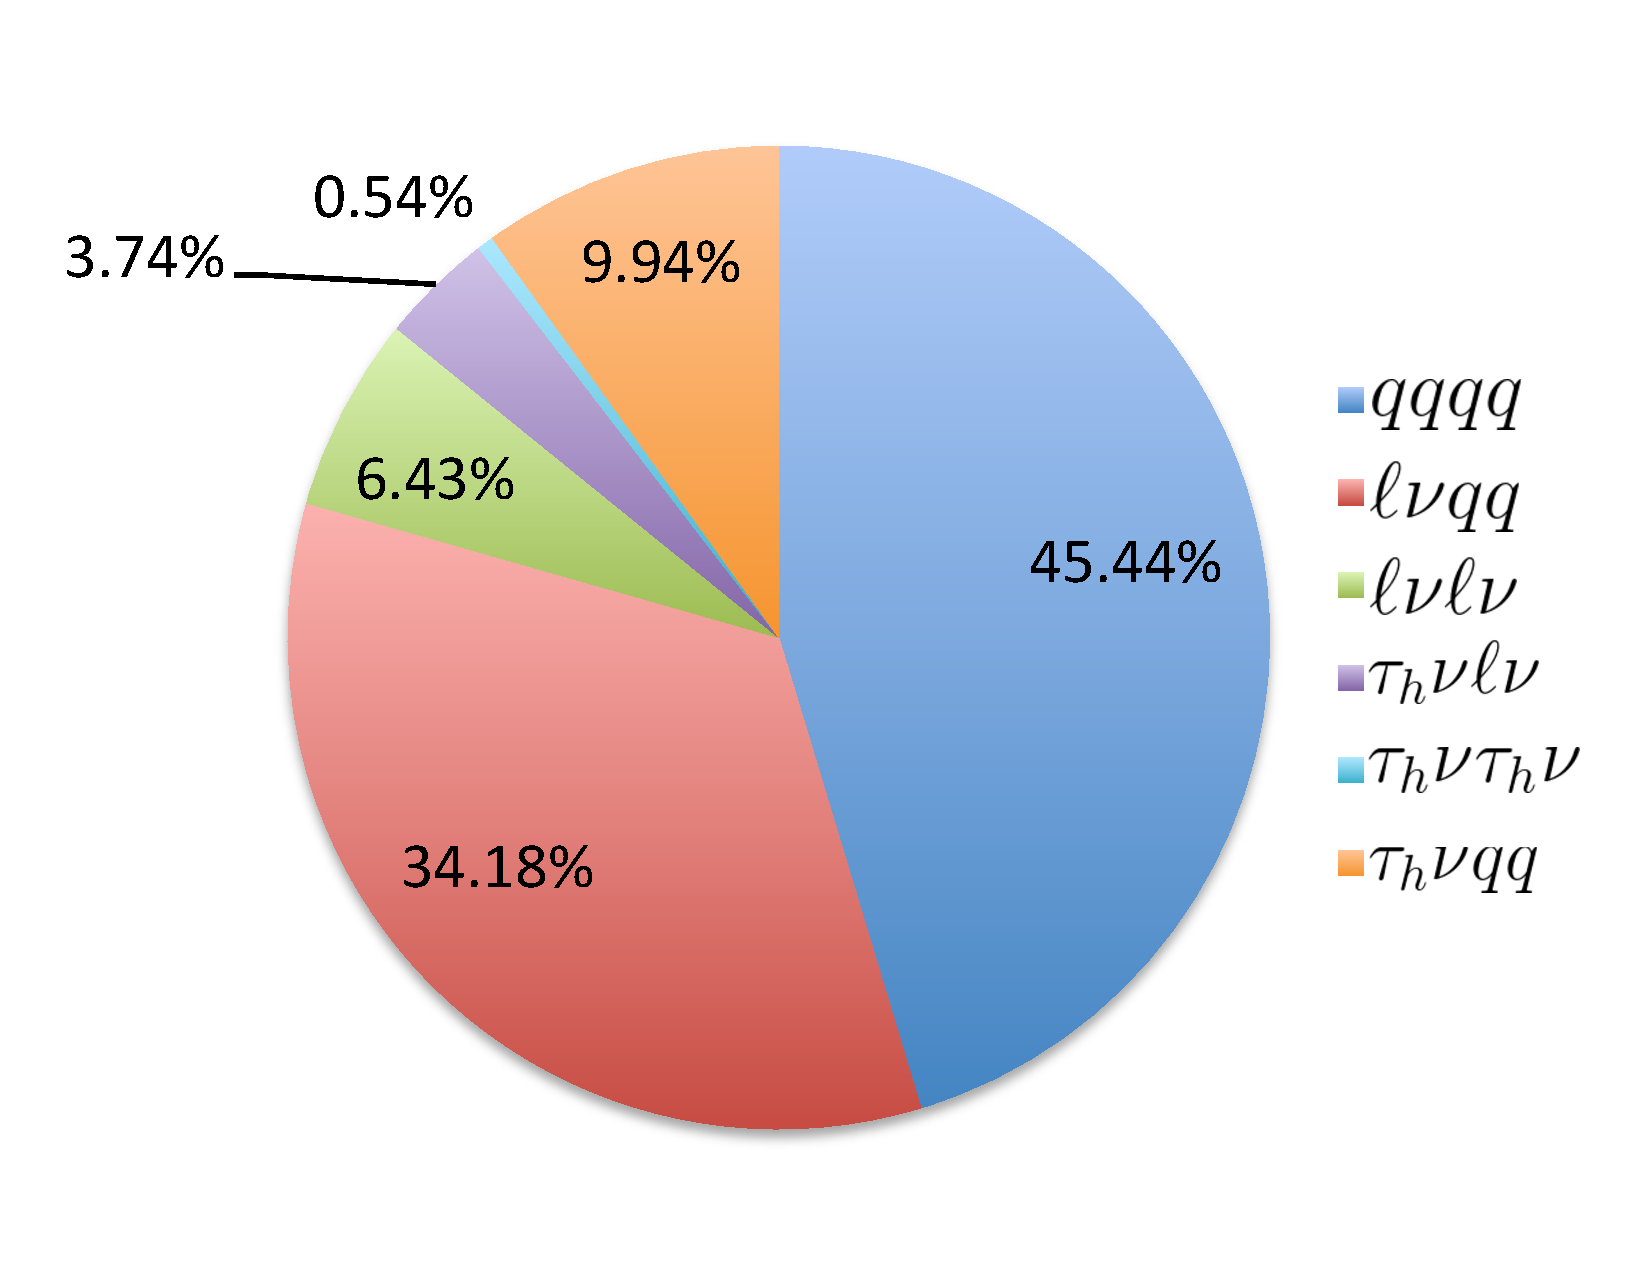
\includegraphics[width=0.7\textwidth]{figures/WWBR}
  %\vspace{-20pt}
  \caption{Branching ratios for a $WW$ system. $q$ refers to quarks. $\ell$ can be either an electron or muon, and the leptonic branching ratios of the $\tau$ are included. For example, the $\ell\nu qq$ final state includes one $W$ decaying to $e\nu$, $\mu \nu$, or $\tau \nu$. $\tau_h$ refer to hadronic decays of the $\tau$.}
  \label{fig:WWBR}
\end{figure}


Figure~\ref{fig:WWBR} shows the relative branching fractions for the $\HWW$ process, calculated from the Particle Data Group values for the $W$ and $\tau$ branching ratios~\cite{PDG}. The largest branching ratio corresponds to both $W$ bosons decaying to quark pairs at 45.44\%. The second largest ratio is for one $W$ decaying leptonically and the other decaying to quarks, a branching ratio of 34.18\%. In all cases, $\ell$ denotes either an electron or muon, and the leptonic branching ratios of the $\tau$ are included. For example, the $\ell\nu qq$ final state includes one $W$ decaying to $e\nu$, $\mu \nu$, or $\tau \nu$. In the case of the $W\to\tau\nu$ decay, the $\tau$ lepton then decays to an electron or muon via $\tau \to \nu_\tau \ell \nu_\ell$. Final states with a $\tau_h$ refer to hadronic decays of the $\tau$. The branching ratio of the $\ell\nu\ell\nu$ final state is 6.43\%. 

While the $\ell\nu\ell\nu$ final state is not a large fraction of the branching ratio, there are significant advantages to using this channel in an analysis. First, both the $qqqq$ and $\ell\nu qq$ channels suffer from a large QCD multijet background, which is often difficult to model. Second, events in the the $\ell\nu\ell\nu$ channel in data can be triggered more efficiently due to the presence of two leptons. 

\section{Background processes}

Many processes from the Standard Model can also produce a final state with two leptons and missing transverse momentum. This section describes the dominant backgrounds to Higgs production and further explains how they can be reduced. Table~\ref{tab:bkgtable} summarizes the different background processes. 

\subsection{Standard Model WW production}

\begin{figure}[h!]
  %\vspace{20pt}
  \centering
  \captionsetup{justification=centering}

  %\hspace*{-32pt}
  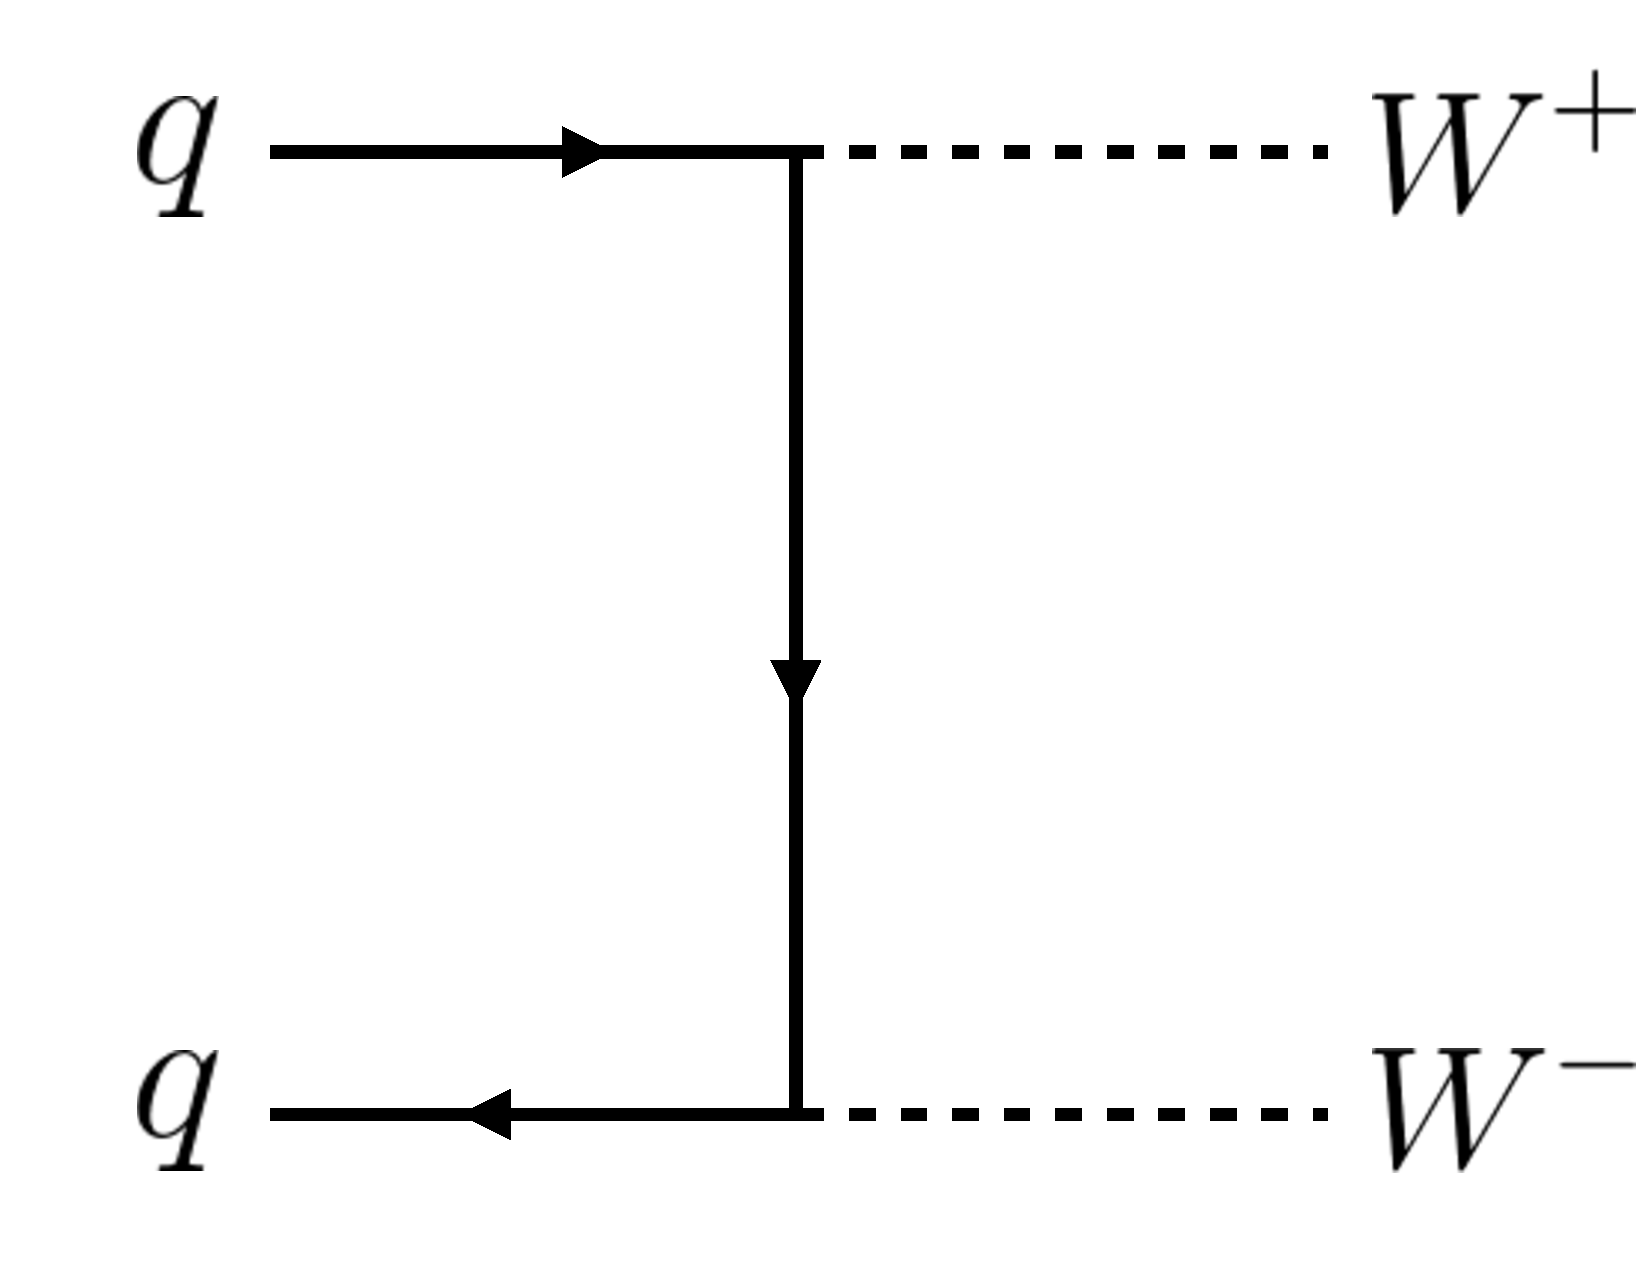
\includegraphics[width=0.3\textwidth]{figures/Feyn_SMWW}
  \caption{Feynman diagram for Standard Model WW production}
  \label{fig:SMWWdiagram}
\end{figure}

Non-resonant Standard Model diboson production, as shown in figure~\ref{fig:SMWWdiagram}, is an irreducible background to Higgs boson production in the WW final state. It produces the same exact final state objects, namely leptonically decaying W bosons. There are no additional objects in the final state that allow for background reduction. Therefore the analysis solely relies on the correlations between the leptons to reduce this background. 

\subsection{Top quark production}

Top quark production can mimic the Higgs in the $WW^*$ final state as well. Top quarks can be produced either in pairs ($\ttbar$ production) or singly ($s$-channel, $t$-channel, or associated production $Wt$). The dominant top background are $\ttbar$ and $Wt$ production.

Because top quarks decay via $t\TO Wb$, top pair production can produce a final state with two W bosons that then decay leptonically. In $Wt$ production, there are two real $W$ bosons produced, as with $\ttbar$. In both cases, there is at least one $b$-jet in the final state. By vetoing on the presence of $b$-jets, these top quark backgrounds can be reduced. Figure~\ref{fig:Topdiagram} shows the Feynman diagrams for $\ttbar$ and $Wt$ production.  

\begin{figure}[h!]
  %\vspace{20pt}
  \centering
  \captionsetup{justification=centering}

  %\hspace*{-32pt}
  \raisebox{-0.5\height}{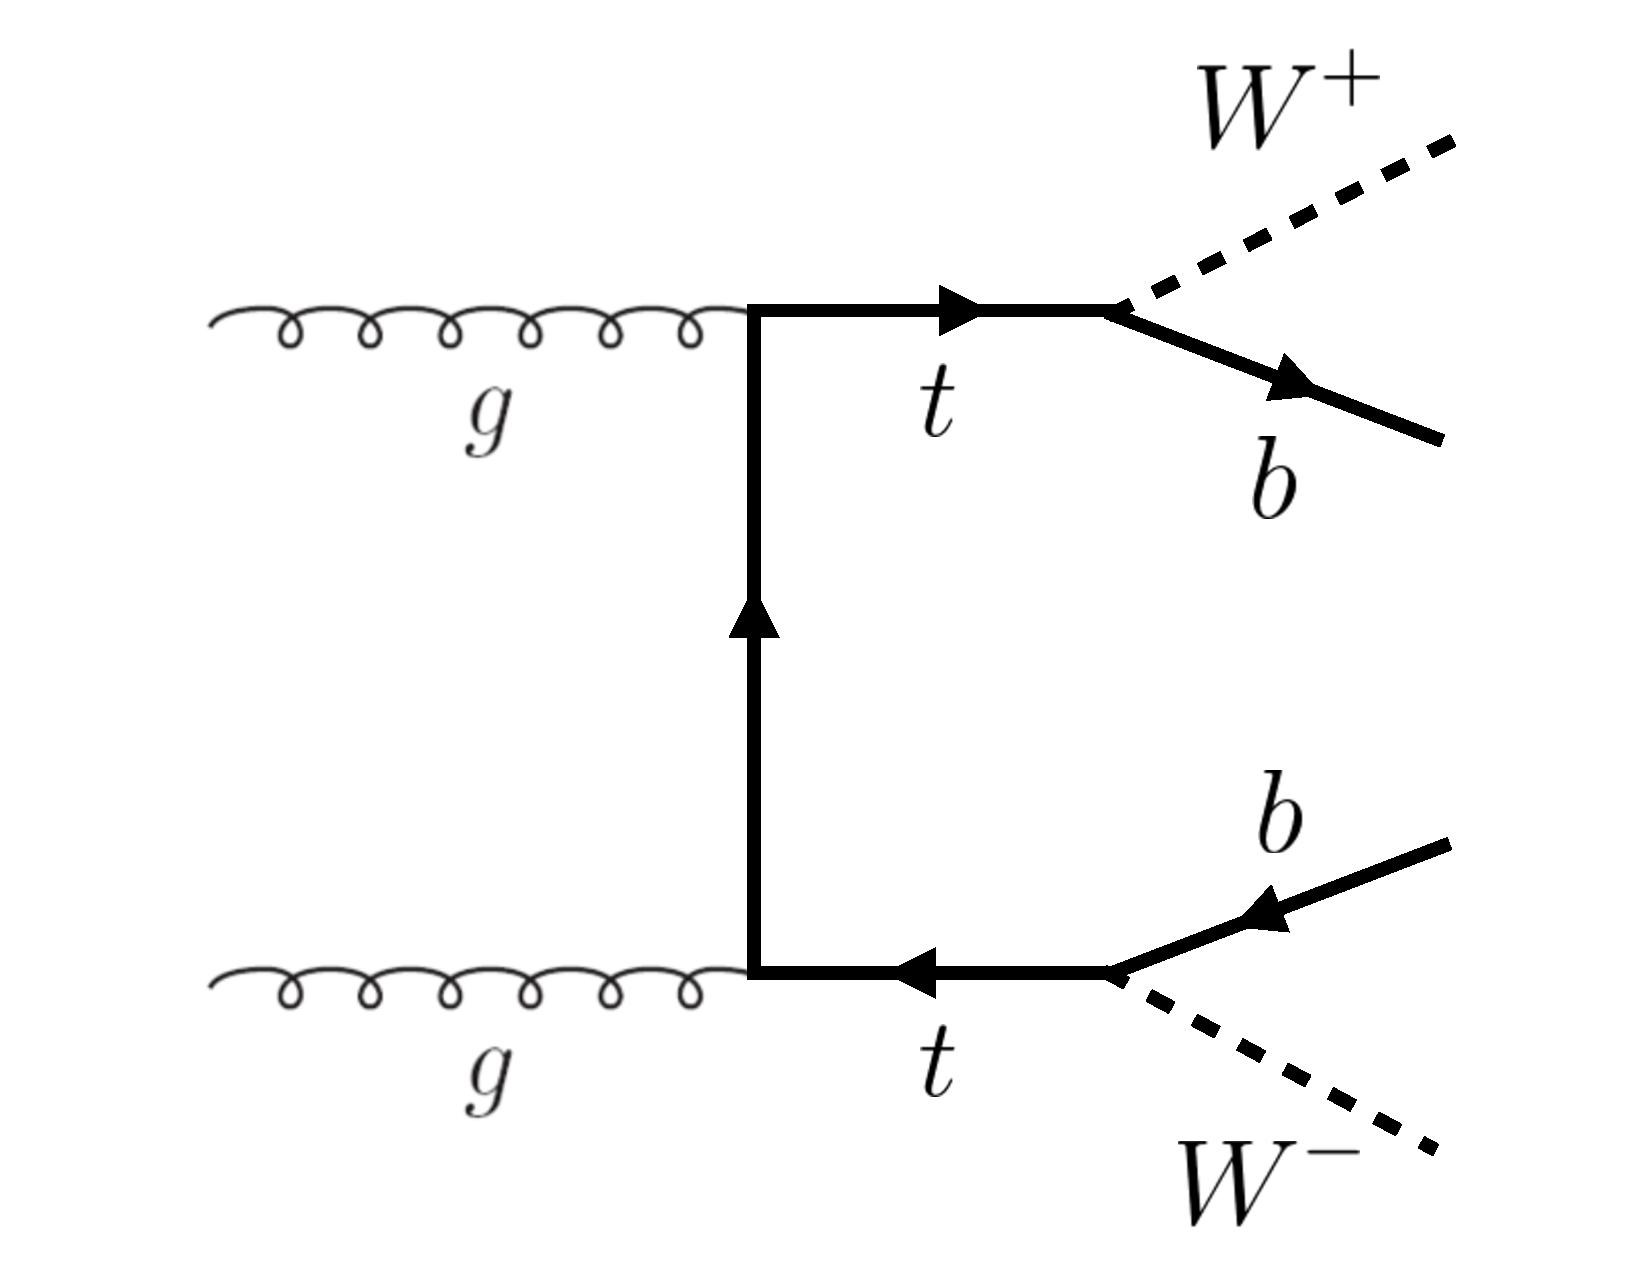
\includegraphics[width=0.3\textwidth]{figures/Feyn_ttbar}}
  \hspace{20pt}
  \raisebox{-0.5\height}{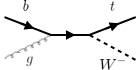
\includegraphics[width=0.3\textwidth]{figures/Feyn_Wt}}
  \caption{Feynman diagrams for top pair production (left) and $Wt$ production (right)}
  \label{fig:Topdiagram}
\end{figure}

\subsection{$W$+jets background}

Single $W$ boson production in association with jets is a unique background to Higgs production. The other backgrounds considered thus far have all included two prompt leptons, each decaying from a $W$ boson, in the final state. In $W$+jets production, however, only one reconstructed lepton originates from a $W$. The second reconstructed lepton is either an algorithmic ``fake" or the result of non-prompt decays. In the first case, the lepton is a jet misidentified as a lepton by either the electron or muon reconstruction algorithms. In the second case, the lepton may be a real lepton but coming from semi-leptonic decays of particles inside the shower of the jet. This background can be reduced by requiring that the reconstructed lepton have little activity in the surrounding region of the calorimeter (also known as an ``isolation"). Figure~\ref{fig:Wdiagram} shows the Feynman diagram for $W$+jets production. 

\begin{figure}[h!]
  %\vspace{20pt}
  \centering
  \captionsetup{justification=centering}

  %\hspace*{-32pt}
  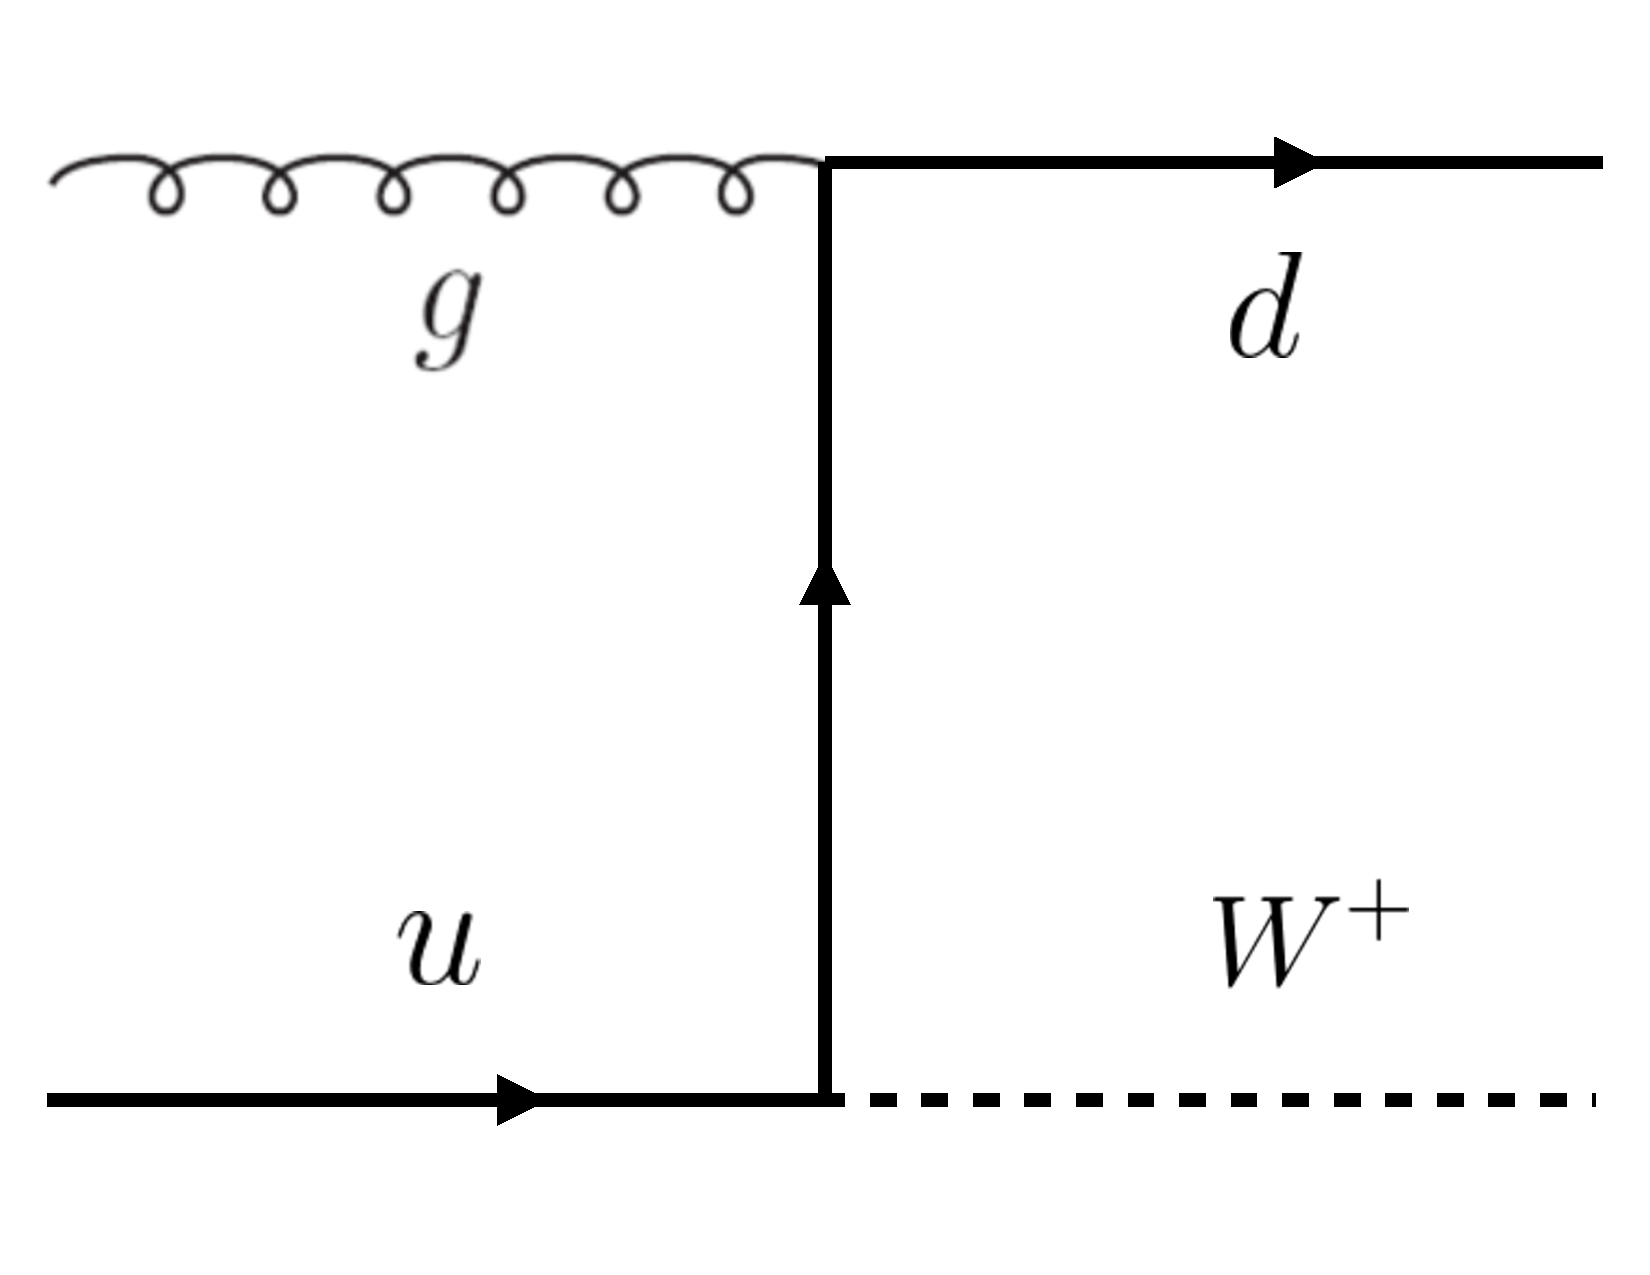
\includegraphics[width=0.3\textwidth]{figures/Feyn_W}
  \caption{An example Feynman diagram of $W$+jets production}
  \label{fig:Wdiagram}
\end{figure}

\subsection{$Z/\gamma^{*}$+jets background}

Production of a $Z$ boson or virtual photon (also known as Drell-Yan and denoted with $Z/\gamma^{*}$) in association with jets is also a background to Higgs production. The $Z$ boson decays to two leptons of the same flavor. When the $\ZDY$ decays directly to electrons or muons, the background enters the same flavor final state. When the $Z$ decays to two $\tau$ leptons the background can enter the different flavor final state as well. Figure~\ref{fig:Zdiagram} shows the production of a $Z$ in association with one jet. Because there are no neutrinos in this final state, variables like $\MET$ can be used to reduce the background\footnote{The $\MET$ cut is much more effective for the reduction of $\ZDY$ production in the same flavor final state. If the background enters the different flavor final state through $\tau$ decays, there will be neutrinos present. Other requirements on the lepton invariant mass are made to reduce the $\ZDY \TO \tau\tau$ background.}. 

\begin{figure}[h!]
  %\vspace{20pt}
  \centering
  \captionsetup{justification=centering}

  %\hspace*{-32pt}
  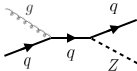
\includegraphics[width=0.3\textwidth]{figures/Feyn_Zjets}
  \caption{An example Feynman diagram of $Z$+jets production}
  \label{fig:Zdiagram}
\end{figure}

\subsection{Subdominant backgrounds}

There are additional processes which contribute to the background composition. These backgrounds are subdominant and contribute less to the total background estimate than those discussed previously. The first process is referred to as $VV$ or ``Other diboson" processes and includes multiple Standard Model diboson processes, including $WZ$, $ZZ$, $W\gamma$, $W\gamma^{*}$, and $Z\gamma$ production. Additionally, there is a background contribution from QCD multijet production. While the cross section for this process is large, its contribution to the $WW^*$ final state is small because two jets must be misidentified as leptons.  

\begin{table}[h!]
\centering
\captionsetup{justification=centering}

%\begin{tabular*}{0.480\textwidth}{p{0.075\textwidth} p{0.180\textwidth} l}
\hspace{-10pt}
%{\renewcommand{\arraystretch}{1.15}
\scalebox{0.9}{
\begin{tabular}{|c|c|c|}
\hline
Category & Process & Description \\ \hline
SM $WW$ & $WW\TO\ell\nu\ell\nu$ & Real leptons and neutrinos \\ \hline
\multirow{3}{*}{Top quark production} & $t\bar{t}\TO WbW\bar{b}\TO\ell\nu b \ell\nu \bar{b}$ & Real leptons, untagged $b$s \\ 
 & $tW \TO WbW \TO \ell\nu\ell\nu b $ & Real leptons, untagged $b$ \\ 
 & $t\bar{b}$, $tq\bar{b}$ & Untagged $b$, jet misidentified as lepton \\ \hline

 \multirow{2}{*}{Drell-Yan} & $\ZDY\TO ee, \mu\mu$ & ``Fake" $\MET$ \\ 
  & $\ZDY\TO \tau\tau \TO \ell\nu\nu \ell\nu\nu $& Real leptons and neutrinos \\ \hline

  \multirow{3}{*}{Other dibosons} & $ZZ \to \ell\ell \nu\nu$ & Real leptons and neutrinos \\ 
   & $W\gamma^{*}, WZ \TO \ell\nu\ell\ell, ZZ \to \ell\ell\ell\ell$ & Unreconstructed leptons \\ 
   & $W\gamma, Z\gamma$ & $\gamma$ reconstructed as $e$, unreconstructed lepton \\ \hline

   $W$+jets & $Wj \TO \ell\nu j$ & Jet reconstructed as lepton \\ \hline
   QCD multijet & $jj$ & Jets reconstructed as leptons \\ \hline
 
 \hline
\end{tabular}
%}
}
%\end{tabular*}
\caption{
  A summary of backgrounds to the \HWWfull signal 
}
\label{tab:bkgtable}
\end{table}


%\section{Object definitions}

%Selecting objects for the analysis is the first step towards rejecting background while maintaining signal acceptance. Details of the object reconstruction algorithms are defined in Chapter 2. This section presents the selections applied for reconstructed electrons, muons, jets, and \met in the final Run 1 \HWWfull analysis in order to 


\section{Shared signal region selection requirements}

As presented in section~\ref{sec:sigtopology}, there are many different combinations of physics objects that can define a \HWWfull final state. The multiplicity of jets and the flavor combinations of the leptons both lead to many potential signal regions. Additionally, signal regions can be optimized separately to be sensitive to the distinct production modes of the Higgs. Gluon fusion, vector boson fusion, and associated production of a Higgs all lead to unique final state topologies. Figure~\ref{fig:analysisregions} delineates the different signal regions used in the gluon fusion and vector boson fusion $\HWW$ analyses. While there are different optimizations possible in each signal region, there are also some commonly shared selections that will be described here.

\begin{figure}[h!]
  %\vspace{20pt}
  \centering
  \captionsetup{justification=centering}

  %\hspace*{-32pt}
  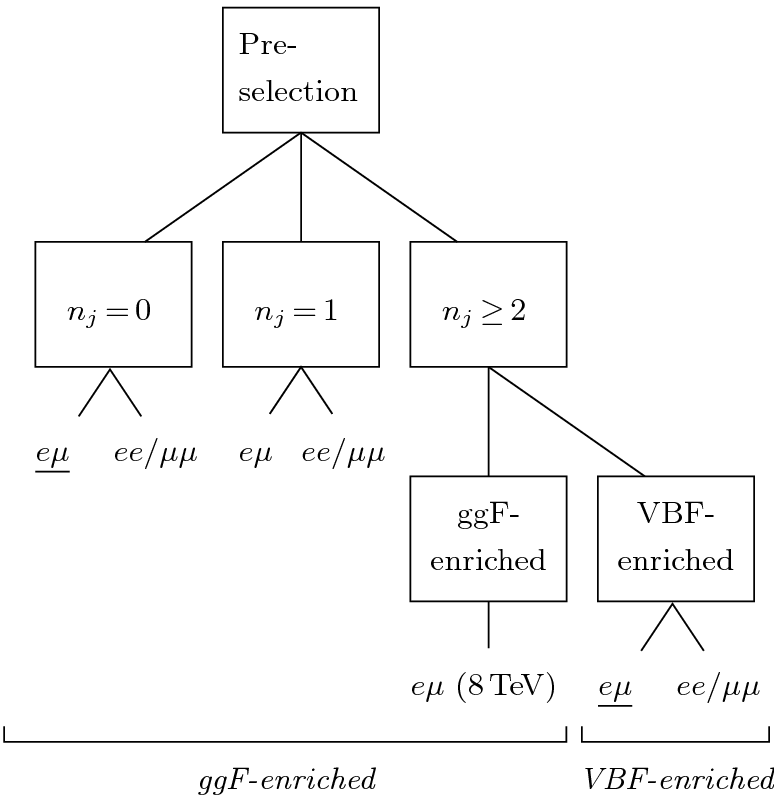
\includegraphics[width=0.6\textwidth]{figures/analysis_regions}
  \caption{An illustration of the unique analysis signal regions~\cite{WW2015}. The most sensitive regions for both gluon fusion and vector boson fusion production are underlined. }
  \label{fig:analysisregions}
\end{figure}

\subsection{Event pre-selection}
\label{sec:HWW_presel}
Before being sorted into the distinct signal regions, basic requirements are applied to the reconstructed objects in the event to select Higgs-like event candidates. First, two oppositely charged leptons are required. Once the leptons are selected, the last requirement for event pre-selection is the presence of neutrinos. As neutrinos cannot be detected directly in ATLAS, $\MET$ can be used as a proxy for the combined neutrino momentum in the transverse plane. 

In general, it is expected that the signal should have a harder $\MET$ spectrum than backgrounds, especially if these backgrounds do not contain neutrinos in the final state. When using $\MET$, it is possible mis-measurements of objects in the detector can lead to imbalances in the transverse plane. When such a mis-measurement occurs, the $\MET$ vector in the transverse plane will often point in the same direction as the mis-measured object. Therefore, a new variable, $\METrel$, is used in the pre-selection. $\METrel$ is defined in equation~\ref{eqn:METrel}. 
%
\begin{equation}
  \begin{array}{ll}
  \multirow{2}{*}{$\METrel$ =\ \bigg\{ }
    &\!\!\!\!\MET\ \sin\dphiNear\quad\textrm{if $\dphiNear<\pi/2$}\\
    &\!\!\!\!\MET\ \phantom{\sin\dphiNear}\quad\textrm{otherwise,}
  \end{array}
\label{eqn:METrel}
\end{equation}
%
If the closest object to the $\MET$ vector is within $\pi/2$ radians in the transverse plane, the $\MET$ is projected away from this object. Otherwise, the normal $\MET$ vector is used. Figure~\ref{fig:METrel} shows a graphical illustration of this concept. 
%
\begin{figure}[h!]
  %\vspace{20pt}
  \centering
  \captionsetup{justification=centering}

  %\hspace*{-32pt}
  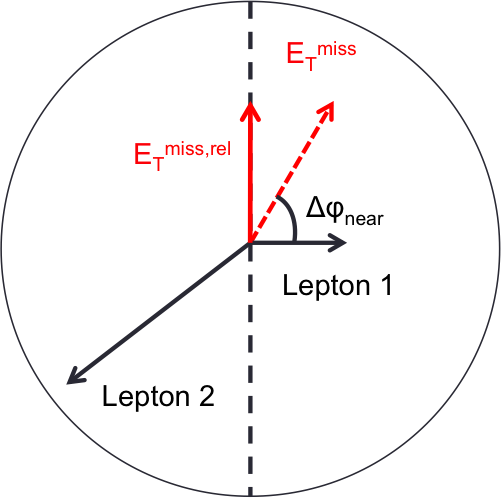
\includegraphics[width=0.6\textwidth]{figures/METrel_cartoon}
  \caption{A graphical illustration of the $\METrel$ calculation}
  \label{fig:METrel}
\end{figure}

Once the lepton and $\MET$ pre-selections are made, the analysis is divided into different regions according to jet multiplicity.

\subsection{Jet multiplicity}
\label{sec:jetmult}
Jet multiplicity, denoted as $\Njet$, is used to sub-divide the analysis into distinct signal regions. By creating separate signal regions, each bin in jet multiplicity becomes sensitive to different modes of Higgs production and different backgrounds.

For example, the $\Njet \geq 2$ region is more sensitive to VBF production because of the two high momentum jets produced at matrix element level. For gluon fusion production to enter this bin, two initial state radiation jets must be emitted. 

Figure~\ref{fig:njet} shows the jet multiplicity in both the different flavor and same flavor regions after the pre-selection. It also shows the background composition in the bins of $\Nbjet$. A few trends from this distribution are worth noting. The first is that the Drell-Yan background dominates in the same flavor channels for $\Njet \leq 1$. Second, the top background becomes a clear contributor to the total background for $\Njet \geq 1$. Lastly, the SM WW production dominates in the $\Njet = 0$ bin, as it is an irreducible background to $\HWW$ production. Because of these distinct features, each jet multiplicity bin is treated separately.

\begin{figure}[h!]
  %\vspace{20pt}
  \centering
  \captionsetup{justification=centering}

  %\hspace*{-32pt}
  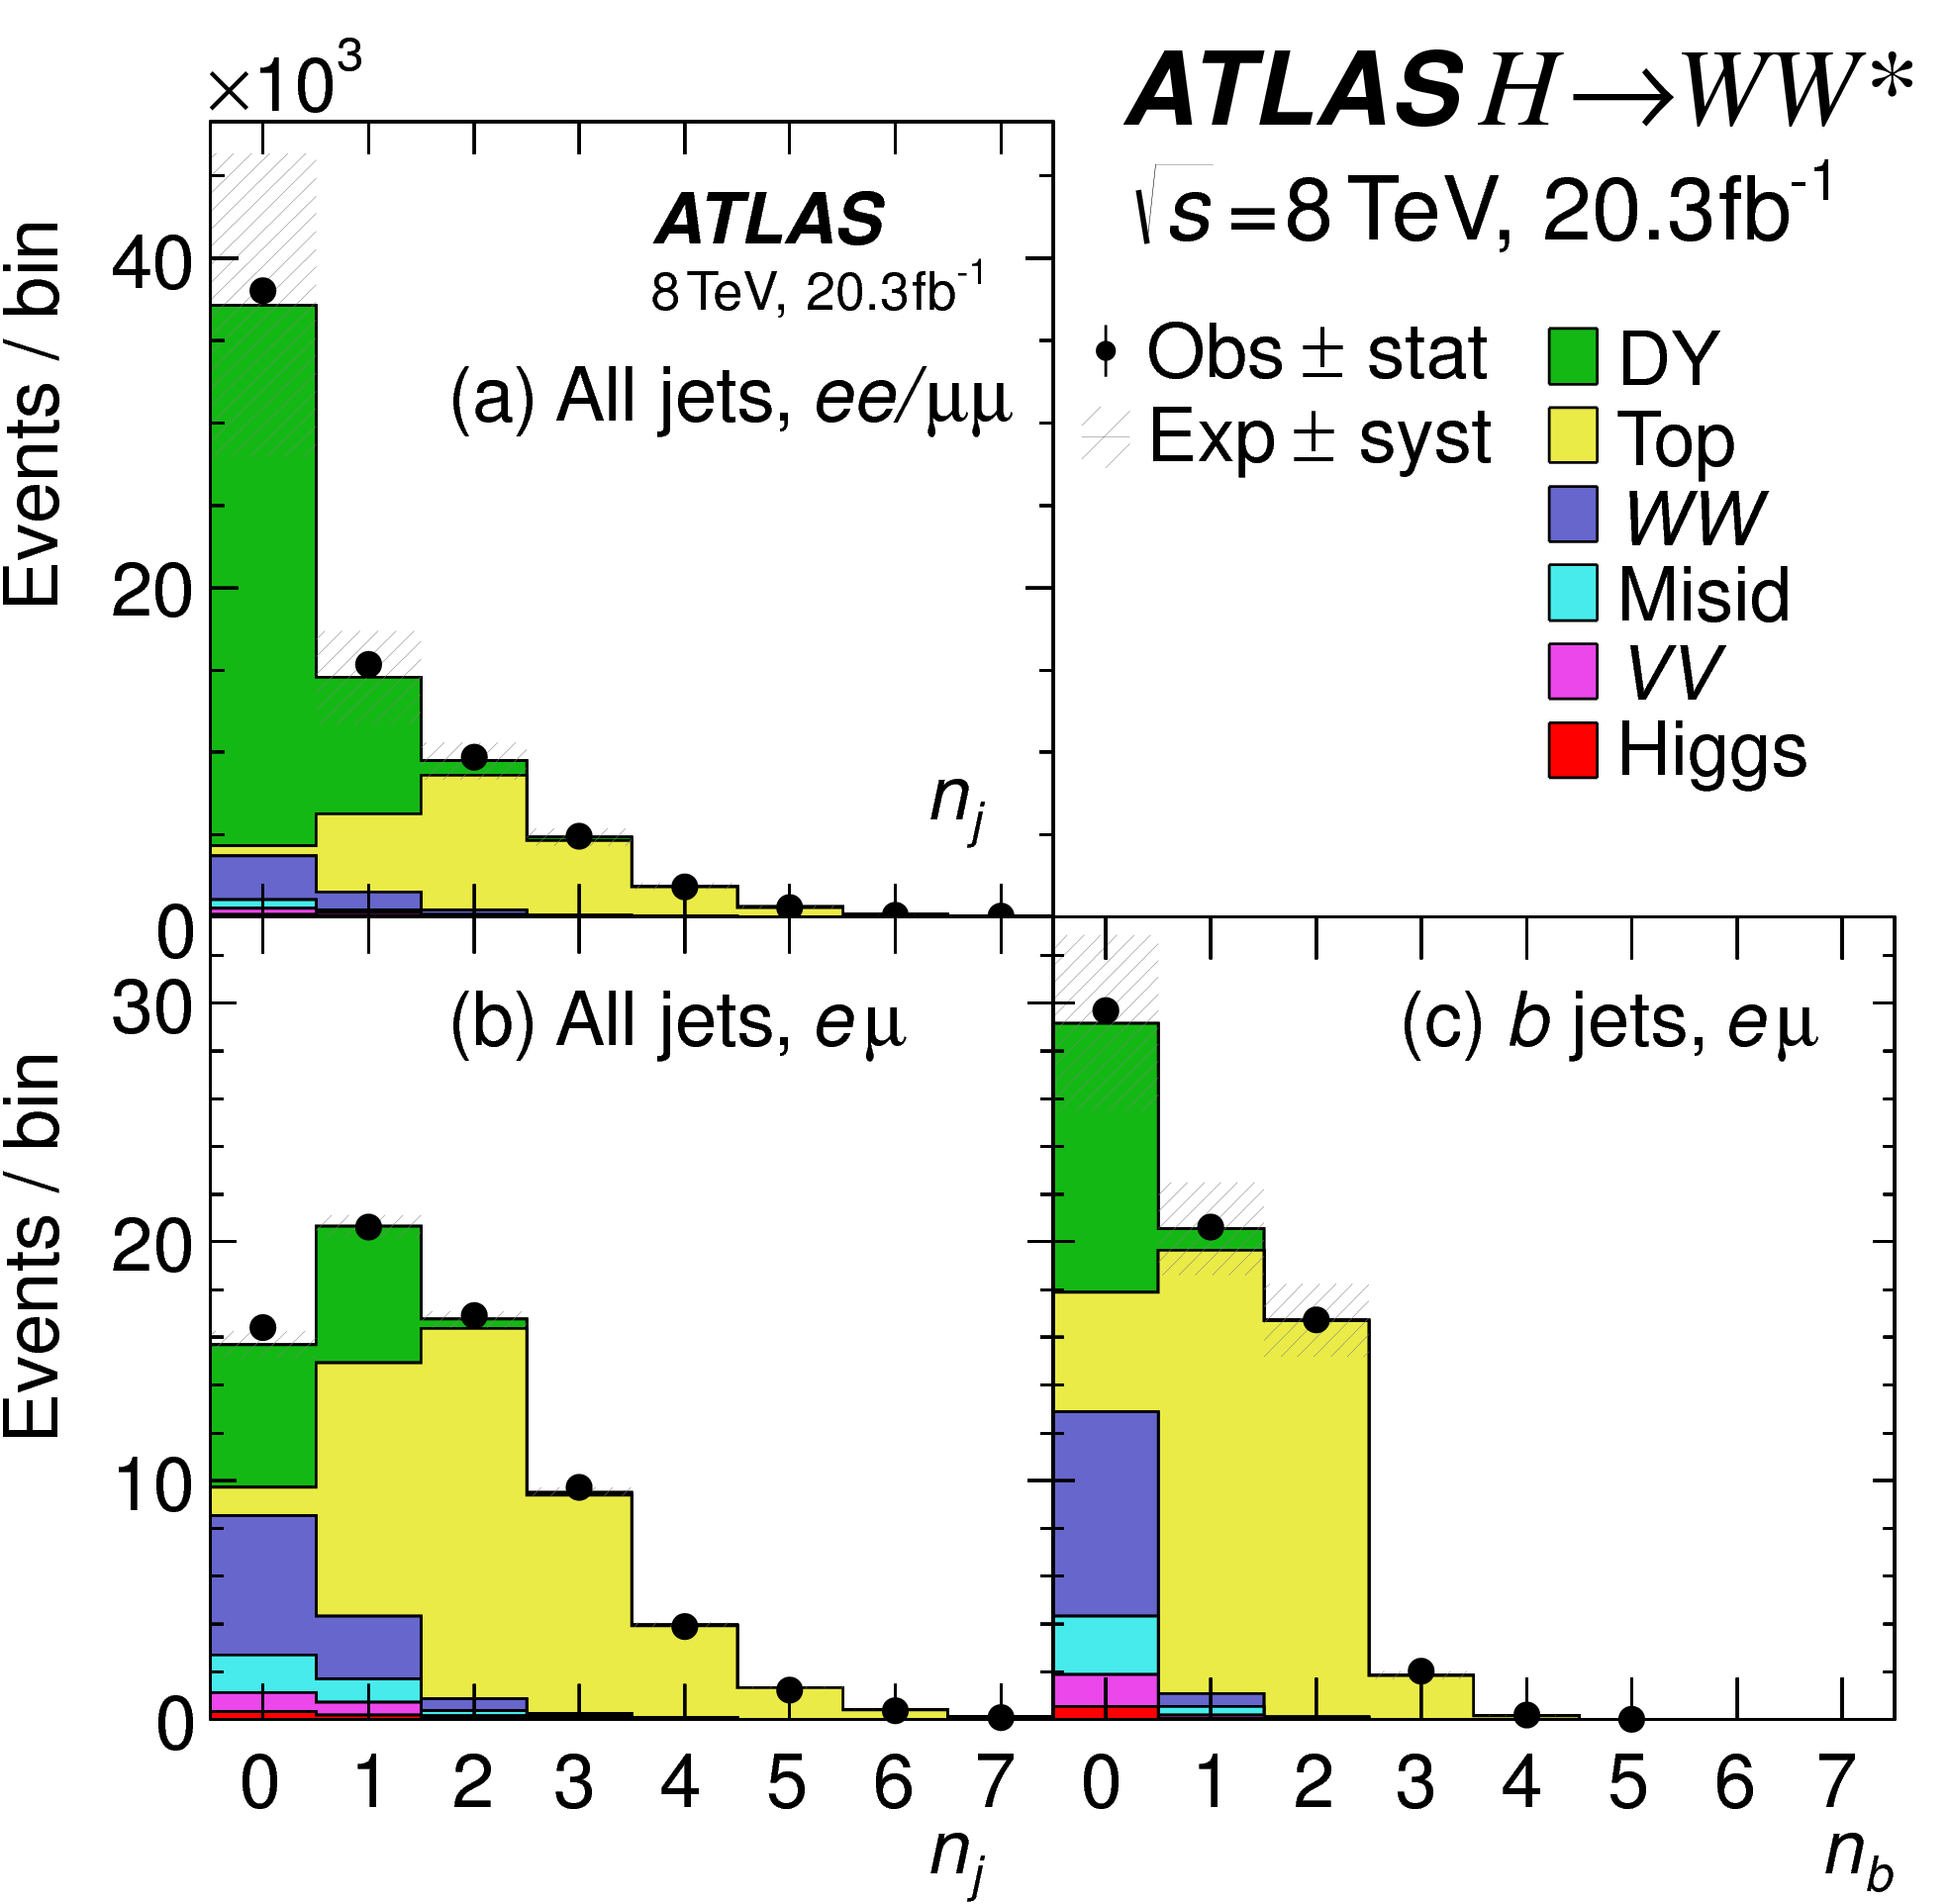
\includegraphics[width=0.6\textwidth]{figures/njet}
  \caption{Predicted backgrounds (compared with data) as a function of $\Njet$ (a and b) and $\Nbjet$ (c) after pre-selection requirements}
  \label{fig:njet}
\end{figure}

\section{Background reduction in same-flavor final states}
\label{sec:sameflavor}
As described in section~\ref{sec:jetmult}, the background composition of the same flavor final states is different from that of the different flavor states. In particular, Drell Yan processes play a much larger role because the $Z/\gamma^{*}$ decays to same flavor leptons. Because real neutrinos are absent in the $\ZDY$ decays to $ee$ and $\mu\mu$, a requirement on $\MET$ should largely reduce the background. However, as this section will demonstrate, with increasing pileup conditions the resolution of the calorimeter-based $\MET$ degrades greatly. Therefore, two new variables for $\ZDY$ background reduction are constructed and described in this section.

\subsection{Pileup and $\MET$ resolution}

Secondary interactions of protons in the colliding bunches of the LHC (known as pileup interactions, described in detail in Chapter 2) deposit energy into the ATLAS calorimeter in addition to the energy that comes from the hard scatter process of interest. The calculation of $\MET$ is fundamentally Poissonian. Summing up all of the energy deposits in individual calorimeter cells or clusters is similar to a counting experiment. The error on a mean of $N$ in a Poisson distribution is $\sqrt{N}$, so the energy resolution scales as $\sqrt{E}$. As more energy is deposited in the calorimeter, the $\MET$ resolution degrades, meaning that the $\MET$ resolution is particularly sensitive to LHC instantaneous luminosity conditions. 

Figure~\ref{fig:Zjetseventdisplay} shows an event display of a $\ZDY$ + jets event candidate with the twenty-five reconstructed primary vertices. This display illustrates that while the interaction of interest only has tracks coming from the hardest primary vertex, all of the secondary interactions  deposit energy in the calorimeter as well.

\begin{figure}[h!]
  %\vspace{20pt}
  \centering
  \captionsetup{justification=centering}

  %\hspace*{-32pt}
  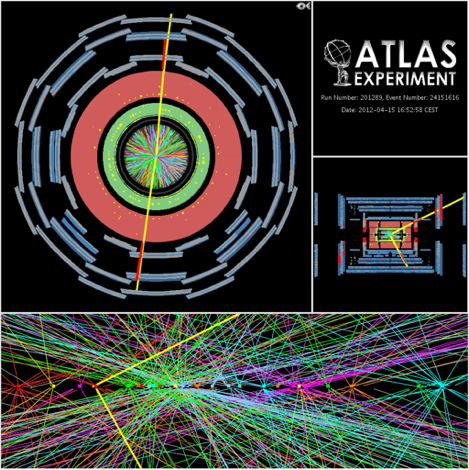
\includegraphics[width=0.6\textwidth]{figures/Zjets_EventDisplay}
  \caption{An event display of a $\ZDY$ + jets event illustrating the effect of pileup interactions}
  \label{fig:Zjetseventdisplay}
\end{figure}

Figure~\ref{fig:METResolution} shows the RMS of the $\MET$ distribution in $Z\TO\mu\mu$ events (where there are no real neutrinos) as a function of the number of the average number of interactions. Under 2011 LHC conditions, this RMS was approximately 9 \GeV, while under 2012 running conditions the resolution worsened to 12 \GeV. The increase in pileup dilutes the $\MET$ variable's ability to reduce the $\ZDY$ background. 

\begin{figure}[h!]
  %\vspace{20pt}
  \centering
  \captionsetup{justification=centering}

  %\hspace*{-32pt}
  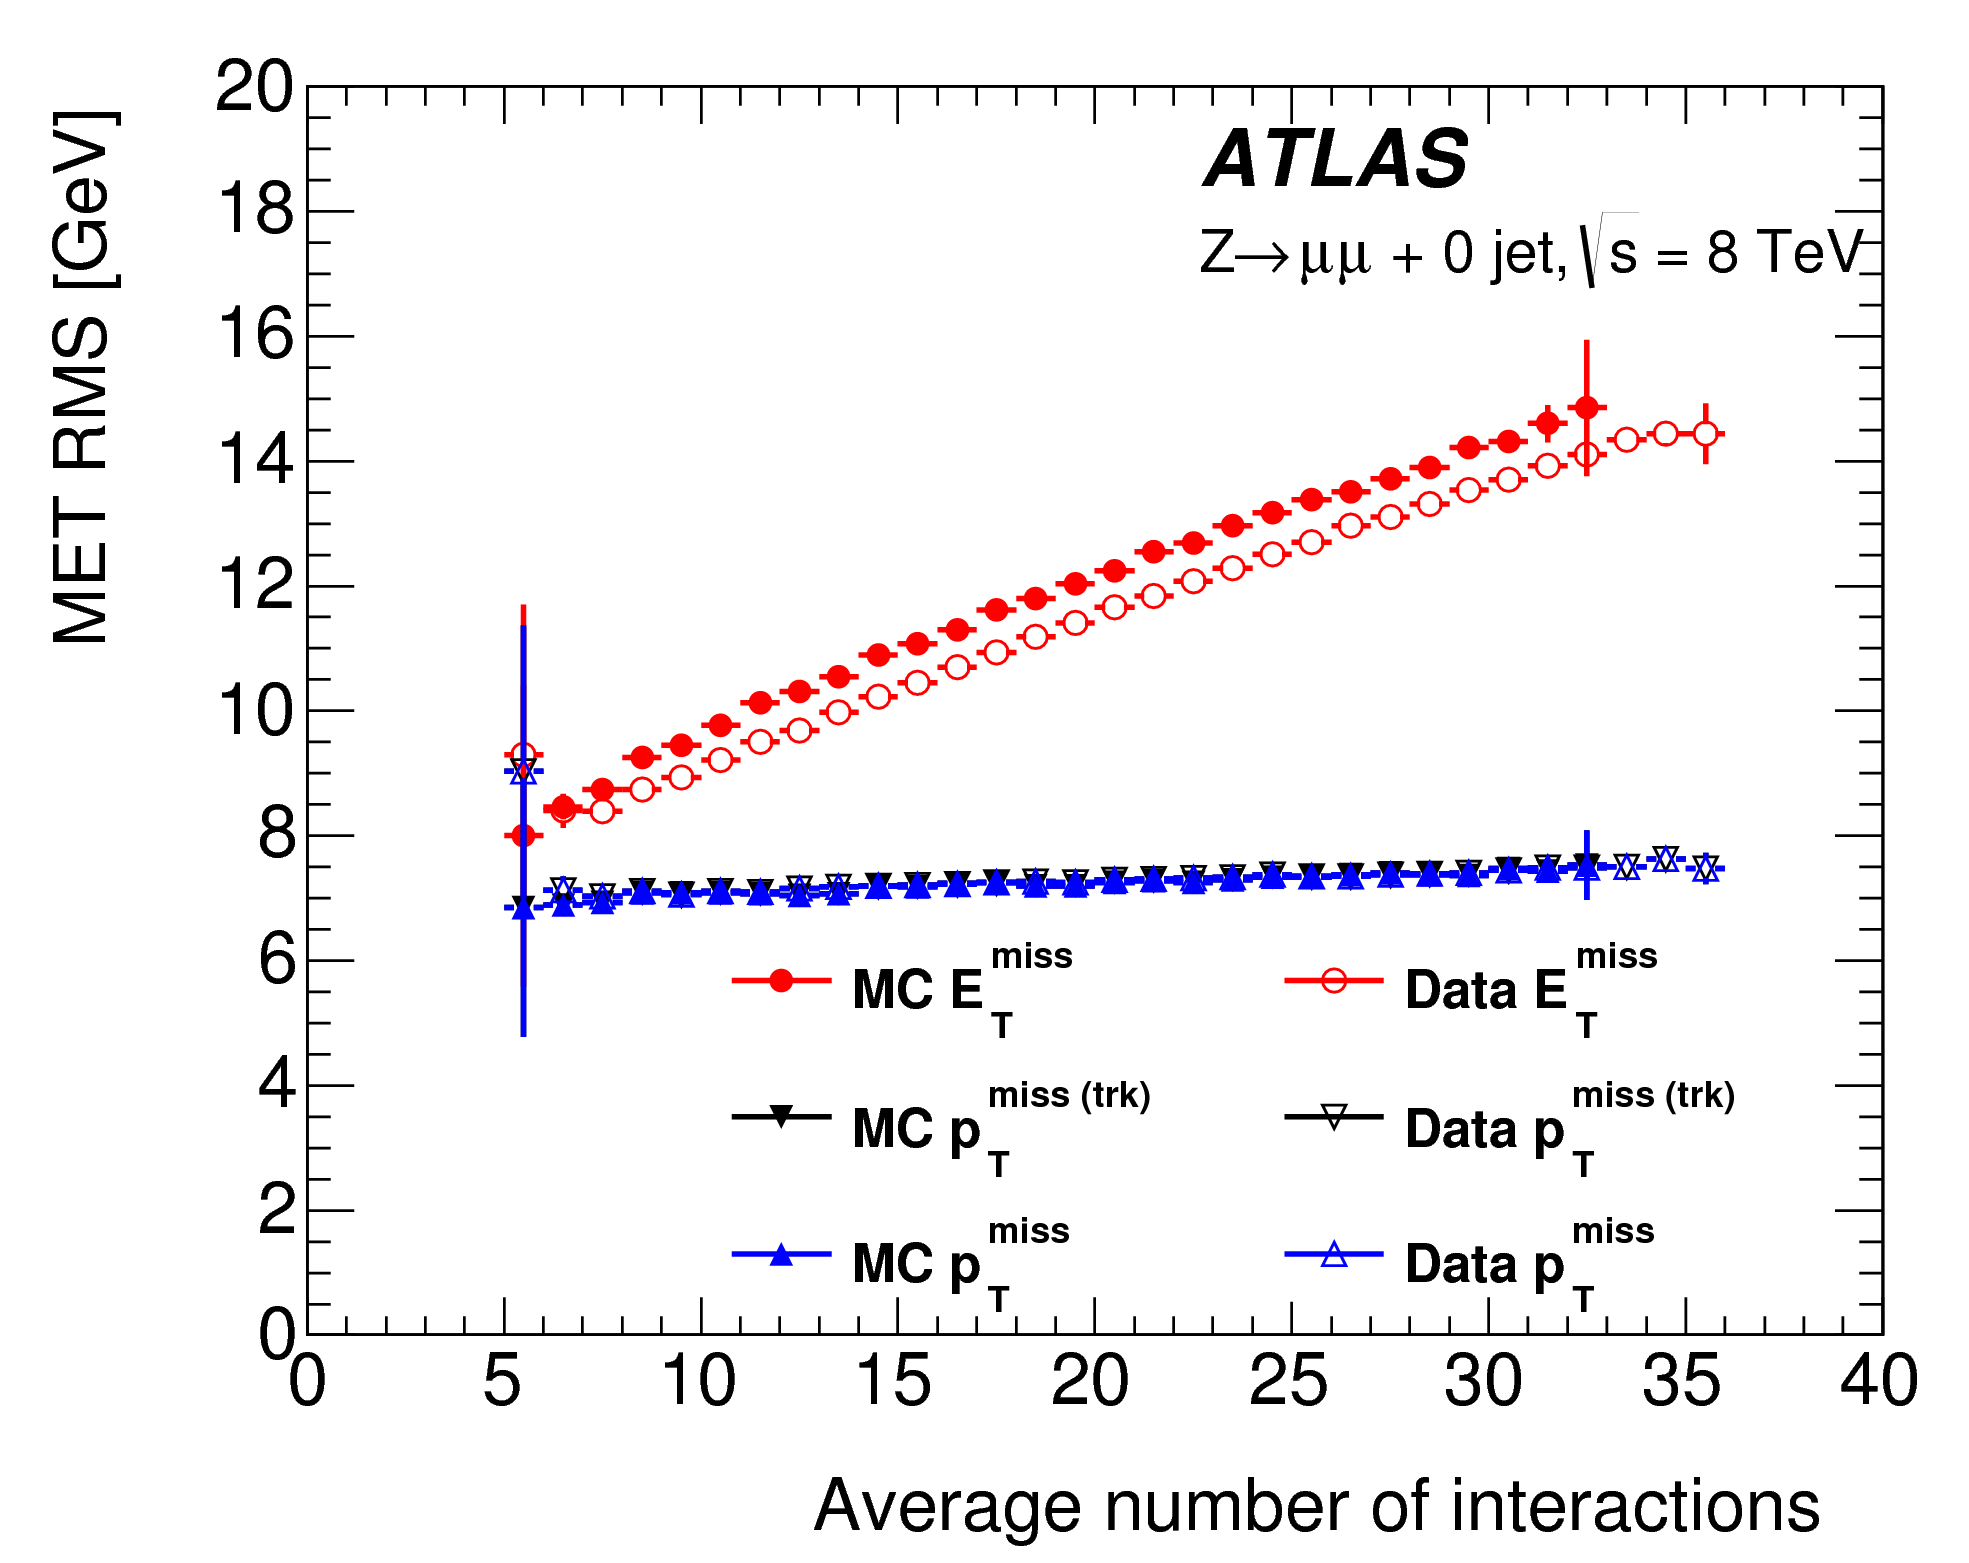
\includegraphics[width=0.6\textwidth]{figures/METResolution}
  \caption{The RMS of different missing transverse momentum definitions as a function of the average number of interactions per bunch crossing}
  \label{fig:METResolution}
\end{figure}

\subsection{Track-based definitions of missing transverse momentum}

Because the increasing number of secondary proton-proton interactions degrades calorimeter-based $\MET$ resolution, a new variable using only contributions from the primary interaction vertex is necessary to further reduce the $\ZDY$ background. While it is not possible to associate calorimeter energy deposits with a particular vertex, individual charged particle tracks in the Inner Detector are associated to unique vertices. Thus, two track-based definitions of \met, using only tracks coming from the primary vertex in the event, are used in the analysis. The simplest variable, $\MPT$, is the vectorial sum of the $\pt$ of all of the tracks from the primary vertex and the selected leptons (excluding the tracks associated with the selected leptons to avoid double counting). Equation~\ref{eqn:MPT} defines $\MPT$.
%
\begin{equation}
\vMPT = -\raisebox{-3.0pt}{\bigg(}%
     \displaystyle
     \sum_{\substack{\rm selected \\ \rm leptons}}\,\vpT
   + \sum_{\substack{\rm other \\ \rm tracks}}\,\vpT
   \raisebox{-3.0pt}{\bigg)},
\label{eqn:MPT}
\end{equation} 
%
To further improve the resolution on the missing transverse momentum, the variable $\MPTj$ is used as defined in equation~\ref{eqn:MPTj}. For selected leptons and jets, the nominal $\pT$ measurements are used. Tracks are used to estimate the soft component of the missing transverse momentum instead of calorimeter measurements. 
%
\begin{equation}
\vMPTj = -\raisebox{-3.0pt}{\bigg(}%
     \displaystyle
     \sum_{\substack{\rm selected \\ \rm leptons}}\,\vpT
   + \sum_{\substack{\rm selected \\ \rm jets}}\,\vpT
   + \sum_{\substack{\rm other \\ \rm tracks}}\,\vpT
   \raisebox{-3.0pt}{\bigg)},
\label{eqn:MPTj}
\end{equation} 
%
Figure~\ref{fig:METResolution} illustrates that these two new variables accomplish their intended purpose. The resolution as a function of mean number of interactions for both $\MPT$ and $\MPTj$ is much flatter than the dependence for $\MET$. 
%
\begin{figure}[h!]
  %\vspace{20pt}
  \centering
  \captionsetup{justification=centering}

  %\hspace*{-32pt}
  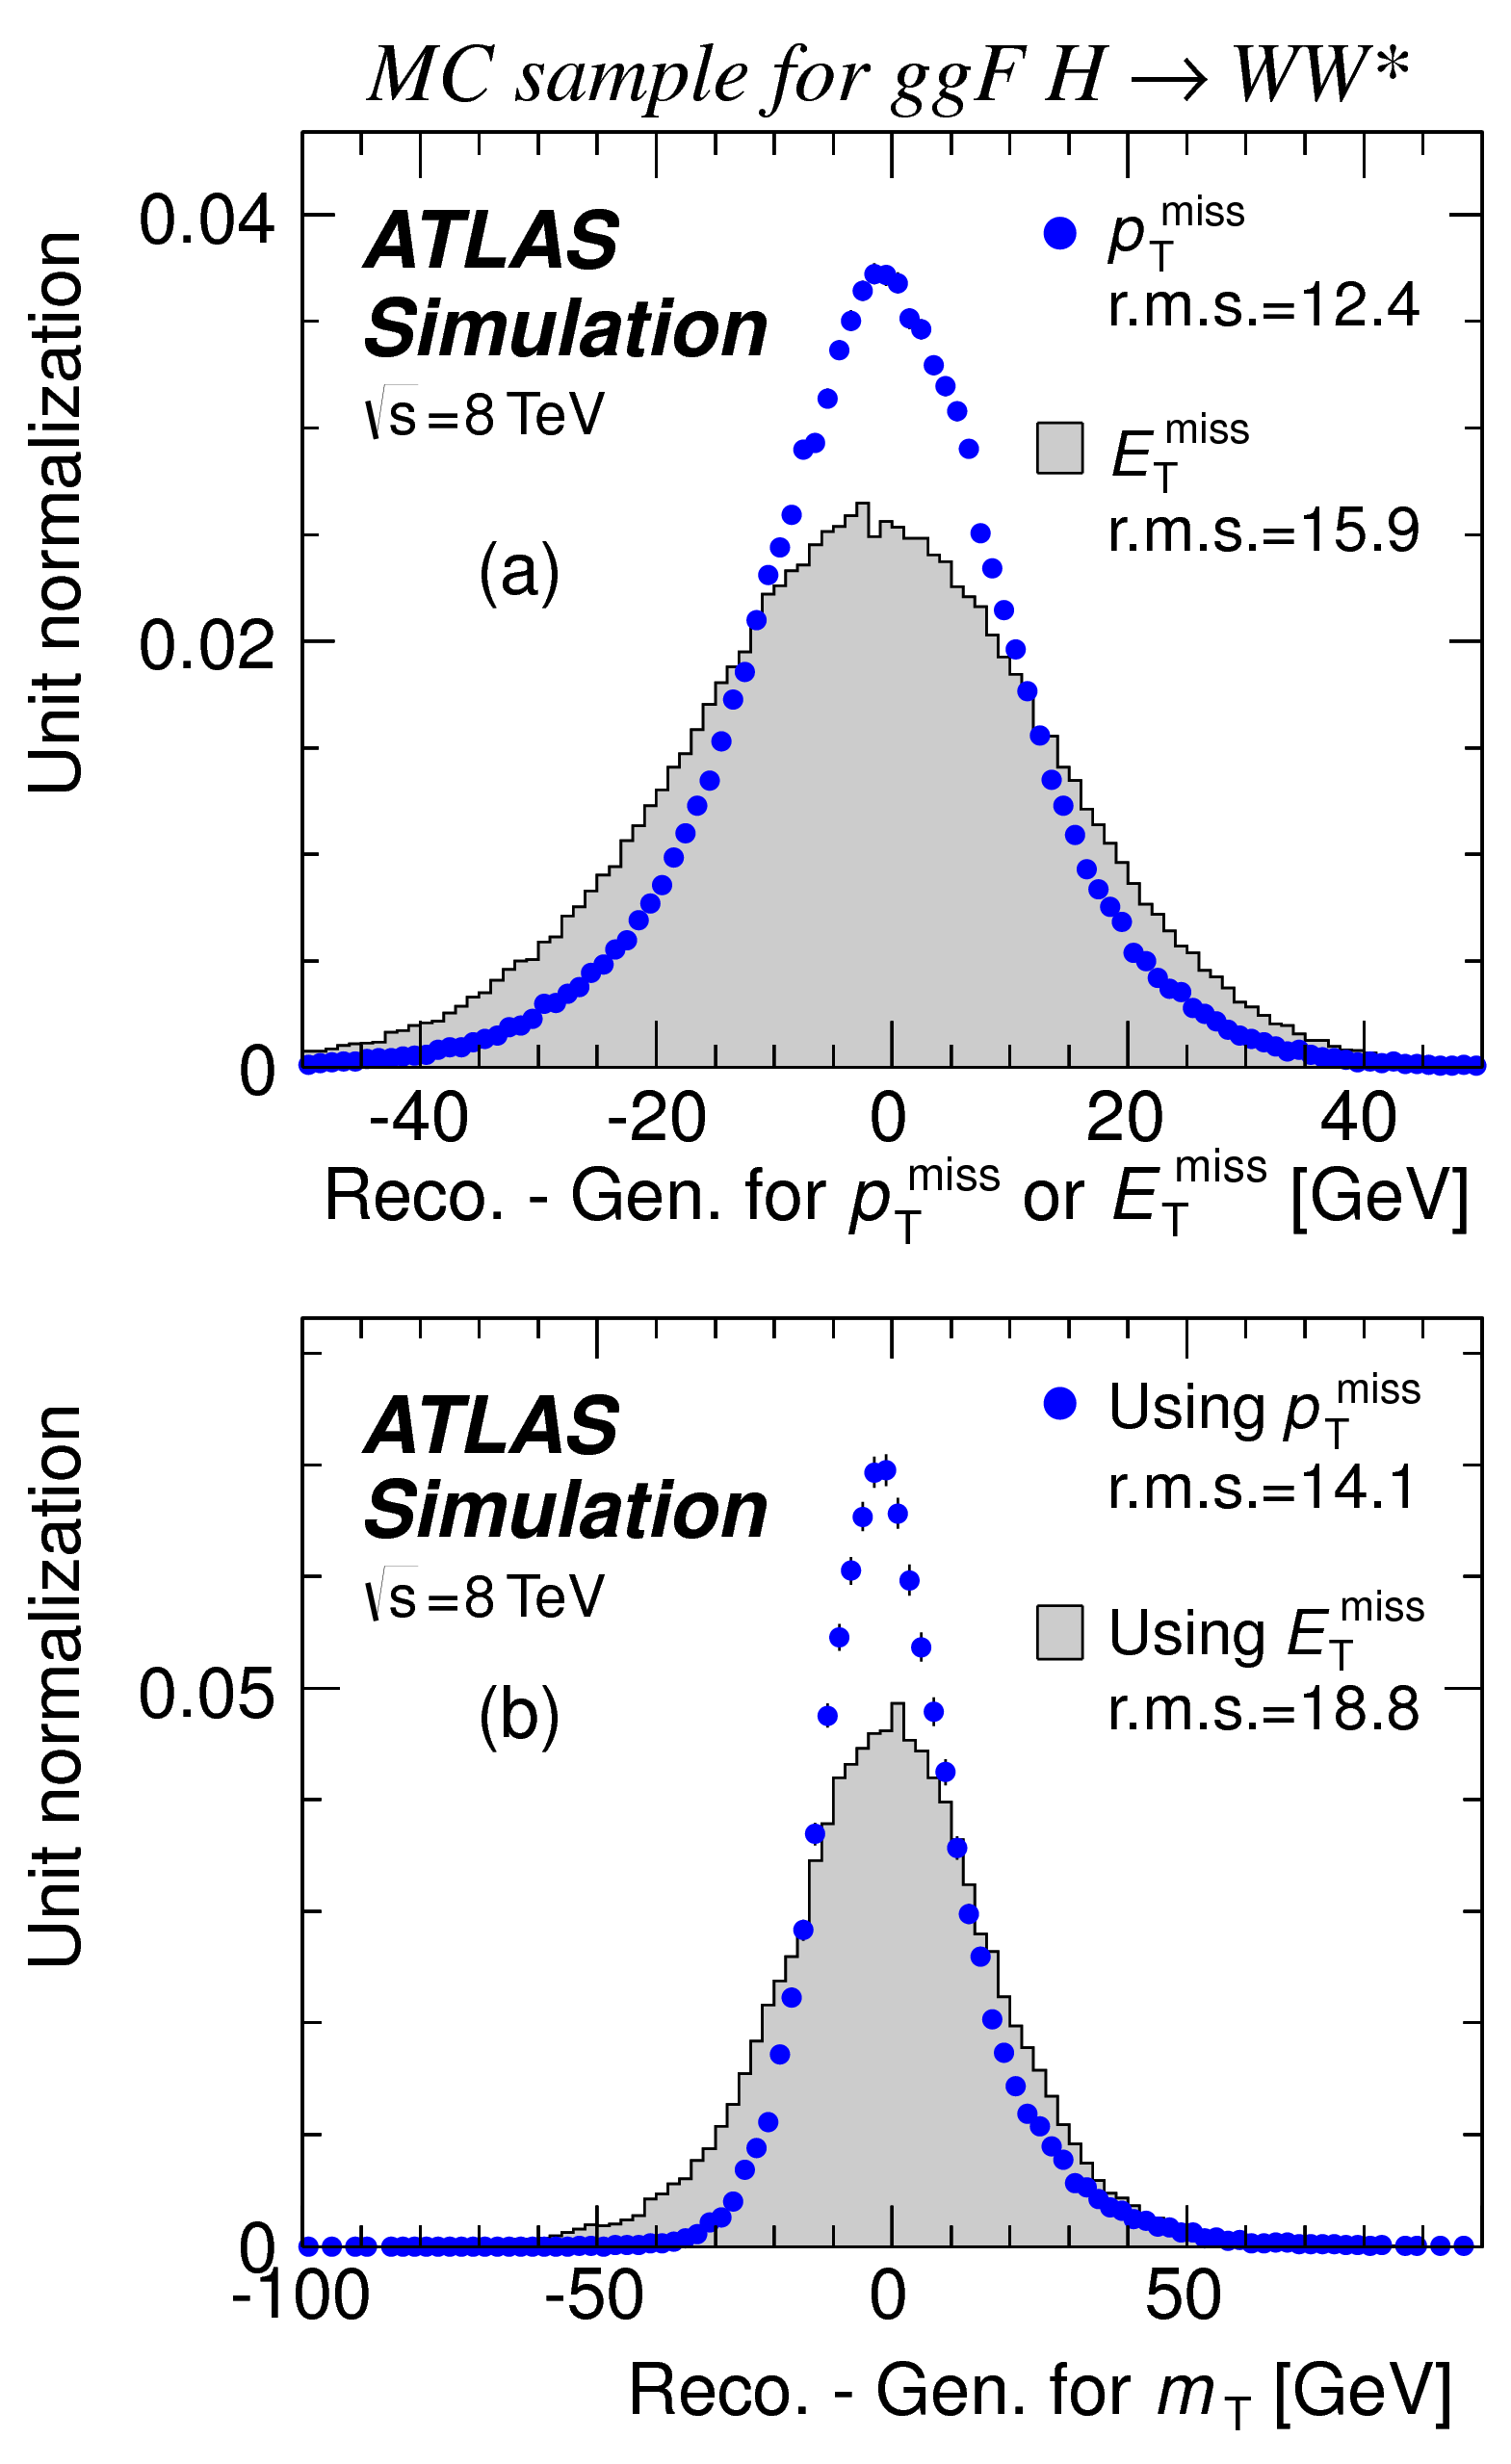
\includegraphics[width=0.6\textwidth]{figures/METResolution2}
  \caption{The difference between the true and reconstructed values of the \met (a) and $\mT$ (b) in a gluon fusion signal sample}
  \label{fig:METResolution2}
\end{figure}
%
Figure~\ref{fig:METResolution2}a shows the difference between the true and reconstructed values of \met using both the track-based $\MPTj$ and calorimeter based $\MET$. The RMS of the distribution improves by 3.5 \GeV when using $\MPTj$.

\subsection{Distinguishing $\ZDY$ +jets and $\HWW$ topologies}

In addition to measuring missing transverse momentum, another variable can be constructed to exploit kinematic and topological differences between the $\ZDY$ background and $\HWW$ signal. Because there are no real neutrinos in the final state (in the case of $Z/\gamma^{*} \TO ee,\mu\mu$ decays), the dilepton system will be balanced with the jets produced in the hard scatter. A new variable, $\frecoil$, is constructed to estimate the balance between the dilepton system and recoiling jets and is defined in equation~\ref{eqn:frecoil}. The transverse plane is divided into four sections, or quadrants, with one quadrant centered on the dilepton vector. The numerator of $\frecoil$ is the magnitude of the vectorial sum of the $\pt$ of jets in the quadrant opposite the dilepton system, weighted by each jet's Jet Vertex Fraction (JVF, described in chapter 2). The denominator is the magnitude of the dilepton $\pt$. 
%
\begin{equation}
\frecoil = \raisebox{-3pt}{\bigg|} \sum_{{\rm jets\,}j{\rm\,in\,}\wedge}
           \no\jvf_{\,j}\cdot\vpTjet
           ~\raisebox{-3pt}{\bigg|}
           ~\raisebox{-3pt}{\bigg/} \pTll.
\label{eqn:frecoil}
\end{equation}
%
Figure~\ref{fig:frecoil} shows a shape comparison of the $\frecoil$ distribution in a simulated $\ZDY$ + jets sample, a $\HWW$ signal sample, and other backgrounds that contain real neutrinos. The $\ZDY$ + jets events tend to be more balanced between the dilepton system and recoiling jets, while the processes containing real neutrinos are less balanced in the transverse plane. Thus, a requirement on $\frecoil$ will reduce the $\ZDY$ + jets background while maintaining a good signal efficiency. 

\begin{figure}[h!]
  %\vspace{20pt}
  \centering
  \captionsetup{justification=centering}

  %\hspace*{-32pt}
  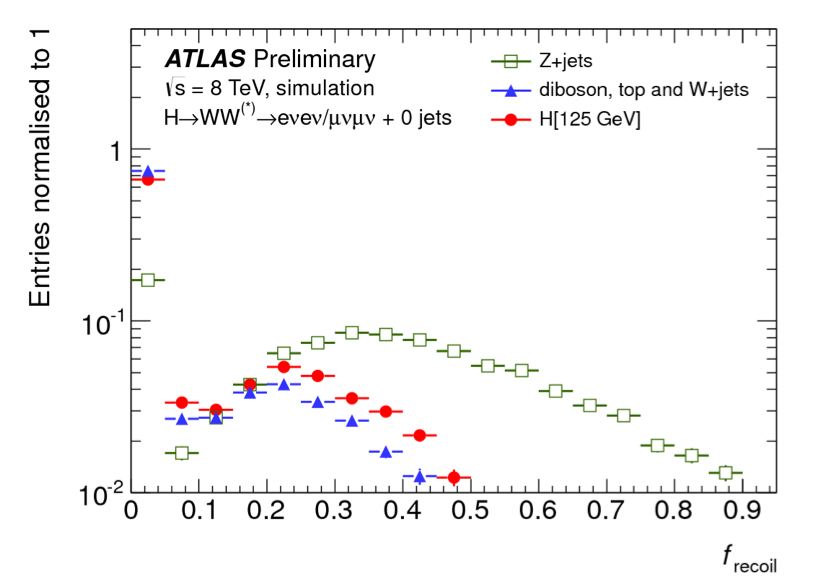
\includegraphics[width=0.6\textwidth]{figures/frecoil}
  \caption{Comparison of $\frecoil$ distributions for $\ZDY$+jets, $\HWW$, and other backgrounds with real neutrinos.}
  \label{fig:frecoil}
\end{figure}

\subsection{Optimizing background reduction selection requirements}

The requirements on $\MPT$ and $\frecoil$ used to reduce the Z+jets background must be optimized to maximize expected signal significance in the same flavor channels. Figure~\ref{fig:optimization} shows an optimization of the combination of the two requirements in the gluon fusion zero jet bin. Each bin shows the expected signal significance if the $\MPTrel$ is required to be greater than the left edge of the bin and the $\frecoil$ is required to be less than the top edge of the bin. The figure shows that the best signal significance comes from requiring low values of $\frecoil$ ($< 0.05$) and $\MPTrel$ values greater than 45 GeV. 

\begin{figure}[h!]
  %\vspace{20pt}
  \centering
  \captionsetup{justification=centering}

  %\hspace*{-32pt}
  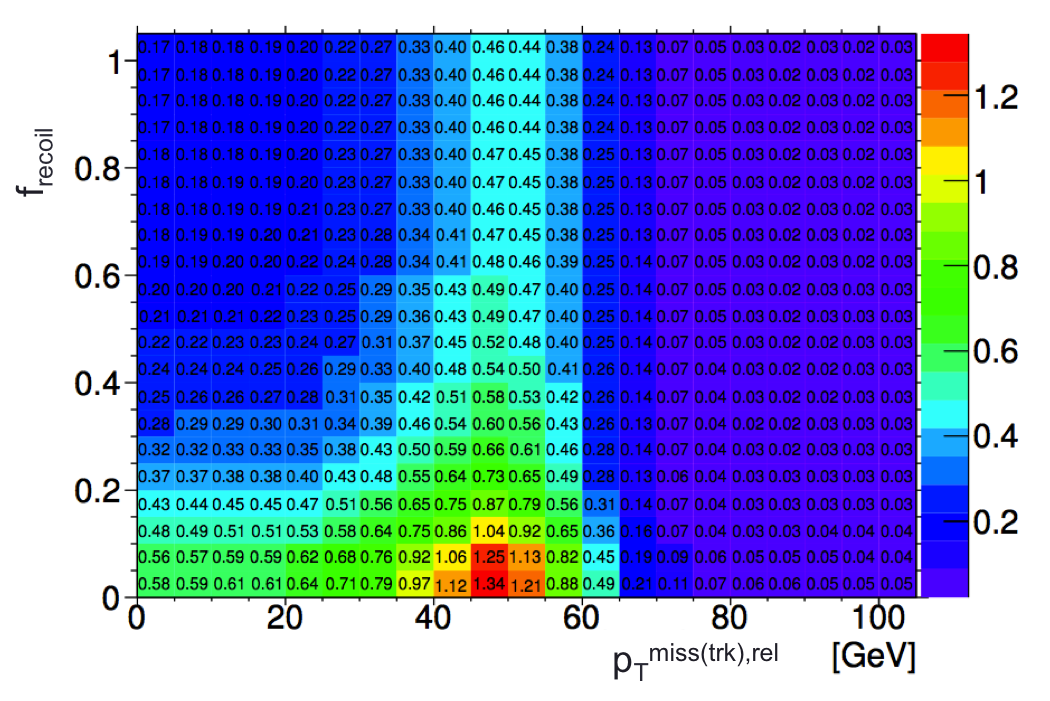
\includegraphics[width=0.8\textwidth]{figures/SFoptimization}
  \caption{Signal significance as a function of required value for $\frecoil$ and $\MPTrel$ in the ggF $\HWW$ with $\Njet = 0$}
  \label{fig:optimization}
\end{figure}


\section{Parameters of interest and statistical treatment}
 
As with any search or measurement, there are particular parameters of the Higgs that the $\HWW$ analysis is interested in measuring. In this case, the parameters of interest are the mass of the Higgs boson and its production cross section. Because the \HWWfull process does not have a closed final state, it is not possible to measure the full invariant mass of the particle that may have produced the final state. However, a proxy for the invariant mass is defined using transverse plane information and detailed in section~\ref{sec:mt}. The second parameter of interest is the ratio of the measured cross section to that expected from the Standard Model Higgs, which is denoted a $\mu$. This is defined in equation~\ref{eqn:mu}.
%
\begin{equation}
\mu = \frac{\sigma}{\sigma_{\rm SM}}
\label{eqn:mu}
\end{equation}
%
All of the likelihoods used in the statistical analysis of the final signal region events are parameterized as a function of $\mu$. $\mu$ is a natural variable for hypothesis testing, as $\mu = 0$ corresponds to a background only hypothesis and $\mu = 1$ corresponds exactly to a Standard Model Higgs. 

\subsection{Transverse mass}
\label{sec:mt}
The \HWWfull analysis cannot reconstruct the full invariant mass of the Higgs because of the neutrinos in the final state. The transverse mass serves as a proxy for the full invariant mass by exploiting information from the transverse plane. The transverse mass is defined in equation~\ref{eqn:mt}.
%
\begin{equation}
  \mTH = \sqrt{\left(\eTll + \MPTj\right)^2 - \left|\,\vpTll + \vMPTj\,\right|^2},
\label{eqn:mt}
\end{equation}
%
Here the $\eTll$ and $\pTll$ are the transverse energy and momentum of the dilepton system, while $\MPTj$ is a proxy for the transverse momentum of the di-neutrino system. The track-based $\MPTj$ is used in the $\mTH$ rather than the calorimeter based $\MET$ because it has a better resolution on the true transverse mass. Figure~\ref{fig:METResolution2}b shows the improvement in the RMS of the difference between the true and reconstructed transverse mass in a ggF signal sample. The RMS improves by 4.7 \GeV using $\MPTj$ in the $\mTH$ calculation.

\subsection[title]{Statistical treatment\footnote{Many thanks to Aaron Armbruster, whose thesis~\cite{ArmbrusterThesis} inspired parts of this section.}}\label{sec:ww_stats}

\subsubsection{Likelihood function}

The statistical analysis of final event candidates is framed as a hypothesis test, where the null hypothesis is background-only (no Standard Model Higgs). The first step in the analysis is to form a likelihood function for the data. In its simplest form, this likelihood is the probability of observing the number of events seen in the final signal region given knowledge of the signal strength. Because observation of events is fundamentally a Poisson counting experiment, this simple likelihood can be expressed as a Poisson probability of observing $N$ events given a total number of predicted signal and background events. This basic likelihood is shown in equation~\ref{eqn:simplepoisson}.
%
\begin{equation}
\likelihood(\mu) = P\left(N | \mu S + B\right)
\label{eqn:simplepoisson}
\end{equation}
%
Here, $P$ is the Poisson probability density function, $N$ is the total number of observed events, $\mu$ is the signal strength, $S$ is the predicted number of signal events, and $B$ is the predicted number of background events. 

In particle physics, certain background estimates are commonly normalized in so-called ``control" regions and those predictions are scaled by the same normalization factor in the signal region. This leads to a slightly more complicated likelihood, which is a function of both the signal strength and the background normalization. This is shown in equation~\ref{eqn:mediumpoisson}.
%
\begin{equation}
\likelihood(\mu, \theta) = P\left(N | \mu S + \theta B\right)P\left(N_{\rm CR} | \theta B_{\rm CR}\right)
\label{eqn:mediumpoisson}
\end{equation}
%
Here, $\theta$ serves as a ``nuisance parameter", or a parameter that is not of primary interest but still enters the likelihood. The second Poisson term enforces that the background normalization be consistent with the number of observed events in data in the control region, $N_{\rm CR}$.

So far, these two formulations of likelihoods have assumed a single signal region and do not take into account any shape information of potential discriminating variables. The $\HWW$ analysis is divided into many different categories, the counting experiment described above can be performed in each individual category. As mentioned in section~\ref{sec:mt}, the transverse mass is used as the primary discriminating variable in many of the $\HWW$ sub-analyses. The same counting experiment can be performed in each bin of the $\mTH$ distribution to incorporate some shape information. Thus, the total likelihood becomes a product over signal regions and bins of the $\mTH$ distribution. Finally, there are usually many backgrounds that are normalized in control regions. The new formulation of the likelihood takes this into account by including a product over control regions in the second Poisson term. All of these modifications are shown in equation~\ref{eqn:binnedpoisson}. 
%
\begin{equation}
\likelihood\left(\mu, \MBF{\theta}\right) = \prod_{\substack{\rm{SRs }\, i \\ \rm{bins }\, b}} P\left(N_{ib} \Bigg| \mu S_{ib} + \sum_{\rm{bkg }\, k}\theta_{k} B_{kib}\right)
 \prod_{\substack{\rm{CRs} \, l}} P\left(N_{l} \Bigg| \sum_{\rm{bkg }\, k}\theta_{k} B_{kl}\right)
\label{eqn:binnedpoisson}
\end{equation}

The final step to obtain the full likelihood used in the analysis is to add nuisance parameters for the systematic uncertainties. In cases where the uncertainty does not affect the shape of $\mTH$ bin-by-bin, each systematic uncertainty $\epsilon$ is allowed to affect the expected event yields through a linear response function of the nuisance parameter, namely $\nu(\theta) = (1 + \epsilon)^\theta$. If instead the uncertainty does affect the shape, the effect is instead parameterized by $\nu_b(\theta) = 1 + \epsilon_{b}\theta$. The value of the nuisance parameters for the systematic uncertainty are constrained with a Gaussian term that is added to the likelihood as well. This is of the form $g(\delta | \theta) = e^{-(\delta - \theta)^2/2}/\sqrt{2\pi}$, where $\delta$ is the central value and $\theta$ is a nuisance parameter. Finally, a last term is added to account for the statistical uncertainty in the Monte Carlo samples used, which adds an additional poisson term. The full likelihood used in the final statistical analysis is defined in equation~\ref{eqn:fullpoisson}.
%
\begin{equation}
\begin{aligned}
\likelihood\left(\mu, \MBF{\theta}\right) = & \prod_{\substack{\rm{SRs }\, i \\ \rm{bins }\, b}} P\left(N_{ib} \Bigg| \mu S_{ib} \cdot \prod_{\substack{\rm{sig.} \\ \rm{syst.} \\ r}} \nu_{br}(\theta_{r})
 + \sum_{\rm{bkg }\, k}\theta_{k} B_{kib} \cdot \prod_{\substack{\rm{bkg.} \\ \rm{syst.} \\ s}} \nu_{bs}(\theta_{s}) \right)
 \\ & \cdot \prod_{\substack{\rm{CRs} \, l}} P\left(N_{l} \Bigg| \sum_{\rm{bkg }\, k}\theta_{k} B_{kl}\right)
 \\ & \cdot \prod_{\substack{\rm syst \\ t}} g\left(\delta_{t} | \theta_{t}\right)
 \cdot \prod_{\substack{\rm bkg \, k}} P\left(\xi_k | \zeta_{k} \theta_{k}\right)
\end{aligned}
\label{eqn:fullpoisson}
\end{equation}
%
The fourth term of the equation quantifyies the uncertainty due to finite Monte Carlo sample size. Here, $\xi$ represents the central value of the background prediction, $\theta$ is the associated nuisance parameter, $\zeta = (B/\delta B)^2$, where $\delta B$ is the statistical uncertainty of $B$.

The best fit value of the signal strength $\mu$ is determined by finding the values of $\mu$ and $\boldsymbol{\theta}$ that maximize the likelihood, while setting $\delta = 0$ and $\xi = \zeta$. Once the likelihood is defined, a test statistic must be built for use in hypothesis testing.

\subsubsection{Test statistic}

To distinguish whether the data match a background only or background and signal hypothesis, a test statistic must be used. The $\HWW$ analysis uses the profile likelihood technique~\cite{Cowan:2010st}. The first step in formulating this test statistic is to define the profile likelihood ratio, shown in equation~\ref{eqn:proflikelihood}.
%
\begin{equation}
\lambda(\mu) = \frac{\likelihood\left(\mu, \hat{\theta}_\mu\right)}{\likelihood\left(\hat{\mu}, \hat{\theta}\right)}
\label{eqn:proflikelihood}
\end{equation}
%
Here $\hat{\theta}_\mu$ is the value of $\theta$ that maximizes the likelihood for the choice of $\mu$ being tested. Additionally, $\hat{\theta}$ and $\hat{\mu}$ represent the values of $\theta$ and $\mu$ that gives the overall maximum value of the likelihood. 

Once this is defined, a test statistic $q_\mu$ is constructed. This is shown in equation~\ref{eqn:qmu}.
%
\begin{equation}
q_\mu = -2 \ln \lambda(\mu)
\label{eqn:qmu}
\end{equation}
%
A higher value of $q_\mu$ indicates that the data are more incompatible with the hypothesized value of $\mu$, and $q_0$ then corresponds to the value of the test statistic for the background only hypothesis. A $p_0$ value is then defined to quantify the compatibility between the data and the null hypothesis. The $p_0$ value is the probability of obtaining a value of $q_0$ larger than the observed value, and this is shown in equation~\ref{eqn:pzero}.
%
\begin{equation}
p_0 = \int_{q_0^{\rm obs}}^{\infty} f(q_\mu | \mu = 0) d q_\mu
\label{eqn:pzero}
\end{equation}
%
Here $f(q_\mu)$ is the probability distribution function of the test statistic. Finally, the $p_0$ value can be converted into a signal significance, using the formula in equation~\ref{eqn:zscore}, or the one-sided tail of the Gaussian distribution. 
%
\begin{equation}
Z_0 = \sqrt{2} \text{erf}^{-1} (1-2p_0)
\label{eqn:zscore}
\end{equation}
%
The threshold for discovery used in particle physics is $Z_0 \geq 5$, more commonly known as a value of $5\sigma$.



